\documentclass[11pt,a4paper]{article}

% ------------------------------ Packages -------------------------------------
\usepackage[margin=1in]{geometry}
\usepackage{microtype}
\usepackage{graphicx}
\usepackage{booktabs}
\usepackage{tabularx}
\usepackage{caption}
\usepackage{float}
\usepackage{enumitem}
\usepackage{amsmath,amssymb}
\usepackage[colorlinks=true,allcolors=blue]{hyperref}
\usepackage[nameinlink,noabbrev,capitalize]{cleveref}

\usepackage{csquotes}
\usepackage[
  backend=biber,
  style=numeric, % simple numeric citations
  sorting=none,
  doi=true,
  url=true,
  eprint=true,
  isbn=true,
  giveninits=true,
  maxbibnames=99
]{biblatex}

\addbibresource{references.bib} % matches .bib filename
\usepackage{pgffor,pgfmath} % for lightweight loops over epochs/layers


% ------------------------------ Setup ----------------------------------------
\setlength{\parskip}{0.5em}
\setlength{\parindent}{0pt}
\graphicspath{{figures/}{.}}

\newcommand{\ProjectName}{POC Multimodal Sparse-MoE}
\newcommand{\ModelName}{Jamba-based Sparse-MoE POC}
\newcommand{\CIFAR}{CIFAR-10}
\newcommand{\AGNEWS}{AG~News}
\newcommand{\MINIUCF}{mini-UCF}
% global tweakable scale for loss curve figures
\newcommand{\LossCurvesScale}{0.50}
% heatmap grid controls (edit to tune layout)
\newcommand{\HeatmapCols}{4}              % images per row
\newcommand{\HeatmapImgWidth}{0.24\linewidth} % width per image (match \HeatmapCols)
% helper: grid of 10 images (single layer)
\newcommand{\HeatmapGridOneLayer}[4]{% baseDir, split(train|val), layerIdx(0), caption
  \begin{figure}[H]
    \centering
    \begin{minipage}{\linewidth}
      \foreach \e in {1,...,10}{%
        \includegraphics[width=\HeatmapImgWidth]{#1/heatmap_epoch\e_layer#3_#2.png}%
        \pgfmathtruncatemacro{\modres}{mod(\e,\HeatmapCols)}%
        \ifnum\modres=0\par\medskip\fi%
      }%
    \end{minipage}
    \caption{#4}
  \end{figure}
}
% helper: grid of 20 images (two layers: 0 and 1)
\newcommand{\HeatmapGridTwoLayers}[3]{% baseDir, split(train|val), caption
  \begin{figure}[H]
    \centering
    \begin{minipage}{\linewidth}
      \foreach \l in {0,1}{%
        \foreach \e in {1,...,10}{%
          \pgfmathtruncatemacro{\t}{int(\l*10+\e)}%
          \includegraphics[width=\HeatmapImgWidth]{#1/heatmap_epoch\e_layer\l_#2.png}%
          \pgfmathtruncatemacro{\modres}{mod(\t,\HeatmapCols)}%
          \ifnum\modres=0\par\medskip\fi%
        }%
      }%
    \end{minipage}
    \caption{#3}
  \end{figure}
}

% ------------------------------ Title ----------------------------------------
\title{\ProjectName: A Minimal Multimodal Language Model with Sparse Mixture-of-Experts and Top-2 Gating}
\author{Stefano Nera \\ Università del Piemonte Orientale, DISIT \\ \texttt{stefano.nera@uniupo.it}}
\date{\today}

\begin{document}
\maketitle

%==============================================================================
\begin{abstract}
This report presents a proof-of-concept multimodal classifier integrating text, image, and video via frozen encoders, concat-projection fusion, and a Sparse Mixture-of-Experts (MoE) block with top-2 routing. The objective is routing correctness and instrumentation—expert counts, load-balance, and top-\textit{k} entropy—under a short training budget with small ablations (experts/layers/capacity).

Results summarize as follows. CIFAR-10 (image + label-derived captions) converges to near-zero train/val loss across all scenarios (e.g., ${\sim}2\times10^{-6}$ by the final epoch), indicating task triviality due to label leakage; it is used primarily to validate routing plots, not to compare accuracy. AG News (text-only, frozen stub encoder) learns quickly then overfits: the best validation loss arrives early (around epoch 5, ${\sim}0.90$) before degrading while train loss continues to fall; MoE width/capacity mainly shift the time-to-plateau rather than generalization, making early stopping essential. On mini-UCF (video + simple text), the small MoE (1 layer, 2 experts) attains the best final validation loss (${\sim}2.15\times10^{-4}$) with slightly higher volatility; the base configuration (2 layers, 4 experts) improves monotonically and finishes close (${\sim}1.8\times10^{-3}$); the wide variant (2 layers, 8 experts) peaks earlier and higher (${\sim}1.65\times10^{-2}$), which shows that assignments are being delayed and reassigned more often; lowering capacity to 1.0 behaves like base, suggesting capacity was not binding at current batch/token settings. Across tasks, load-balance is generally high and top-\textit{k} entropy declines over training; capacity adjustments matter chiefly when expert slots saturate. These outcomes align with the POC intent: validate sparse MoE routing and diagnostics, and expose qualitative effects of topology and capacity under frozen encoders.
\textbf{Tokenizer note:} Text is tokenized with the Jamba tokenizer (\texttt{ai21labs/Jamba-v0.1})\cite{jamba2024} only—no Jamba LM weights are loaded—to standardize tokenization while isolating MoE routing behavior.
\end{abstract}

%==============================================================================
\section{Introduction}
\textbf{Problem.} Multimodal inputs couple heterogeneous statistics (spatial, temporal, lexical) and long-tail correlations, making a single dense pathway sample-inefficient and compute-heavy. Scaling dense Transformers increases FLOPs, activation memory, and bandwidth roughly linearly with depth and quadratically with sequence length; fusion further amplifies these costs by concatenating modality tokens and expanding the KV-cache footprint. In practice, three issues dominate: (i) representation mismatch across modalities (resolution, sequence length, noise) that motivates specialization capacity; (ii) batch and data heterogeneity that induces optimization interference and gradient conflict; and (iii) hardware limits where activation memory and memory bandwidth, not parameter count, become the primary bottlenecks. Sparse MoE addresses these pressures by decoupling parameter count from per-token compute via conditional routing, enabling larger capacity at bounded active FLOPs. Yet sparse systems introduce new failure modes—router instability, expert collapse and load imbalance, capacity-induced overflow/dropping, and sensitivity to batching/tokenization—necessitating explicit balance regularization and fine-grained routing diagnostics.

\textbf{POC goal.} Demonstrate a minimal but instrumented multimodal classifier with sparse MoE and interpretable routing; prioritize correctness and diagnostics over full convergence.

\textbf{Contributions.}
\begin{itemize}[leftmargin=*]
  \item Unified pipeline with frozen text/image/video encoders, concat-projection fusion, and a top-2 routed MoE block with SwiGLU experts.
  \item Instrumentation and plots: expert counts, load-balance, and top-k entropy across tasks and layers.
  \item Scripted scenario sweep via \texttt{run\_different\_training\_scenarios.sh} with per-run plots.
\end{itemize}

\textbf{Scope.} Short training; classification only; text path uses a frozen stub; the video subset is intentionally small to control IO/VRAM.

%==============================================================================
\section{Literature Review}
\subsection{Sparse Mixture-of-Experts Architectures}
Sparse Mixture-of-Experts (MoE) decouples parameter count from per-token compute by routing each token to a small subset of experts. This yields models with substantially larger capacity at roughly constant FLOPs per token, improving the performance–compute trade-off relative to dense baselines \cite{he2024_million_experts,ijcnn2024_efficient_routing}. Recent routing advances further tighten this trade-off: regularized-OT and related load-balancing strategies stabilize token–expert assignment and accelerate convergence \cite{ijcnn2024_efficient_routing}, while thresholded and sparser selection mechanisms reduce unnecessary activations without degrading quality \cite{yang2024_sparser_selection}. Retrieval-style layers that select from very large expert pools extend this idea to extreme scales, maintaining efficient inference while growing capacity \cite{he2024_million_experts}.

Efficiency gains are not limited to compute. Architecture–hardware co-design and structured sparsity enable aggressive compression and power savings; some designs report order-of-magnitude parameter compression \cite{li2018_resource_aware}. Approximations targeting Transformer feed-forward blocks complement sparsity by lowering activation and memory footprints \cite{csordas2023_approx2ffn}. Despite these strengths, MoE systems remain sensitive to routing pathologies. Poorly trained routers can starve experts, harm specialization, and yield unstable training, underscoring the need for explicit load-balance terms and expert-usage diagnostics during optimization \cite{ijcnn2024_efficient_routing,yang2024_sparser_selection}.

\subsection{Multimodal Large Language Models}
Multimodal LLMs (MLLMs) differ from text-only LLMs by integrating modality-specific encoders and cross-modal fusion modules that align non-text features to a language interface. Typical designs pair vision encoders with projection layers and cross-attention or fusion adapters, enabling joint reasoning over text, images, audio, or video \cite{carolan2024_review_mmlm,bai2024_revolution_mllm}. Training stacks extend beyond next-token prediction to include multimodal pretraining, alignment losses, and instruction tuning that standardize input–output formats across modalities \cite{carolan2024_review_mmlm,gargbas2023_performance_mllm,niu2024_data_centric_mllm}.

These architectural differences translate into practical gains: MLLMs achieve stronger performance on tasks requiring cross-modal grounding, compositional reasoning, and zero-shot adaptation than text-only models exposed solely to captions or textual descriptions \cite{gargbas2023_performance_mllm,bai2024_revolution_mllm}. The benefits depend on data coverage and alignment quality; insufficient or biased multimodal corpora can limit generalization and propagate modality-specific biases, particularly in safety-critical domains such as healthcare \cite{niu2024_data_centric_mllm,carolan2024_medical_mllm}.

%==============================================================================
\section{Architecture}
\subsection{System Diagram}
\Cref{fig:system-diagram} summarizes the end-to-end pipeline. Text is tokenized with the Jamba tokenizer (\texttt{ai21labs/Jamba-v0.1})\cite{jamba2024}; the text path is a frozen stub that average-pools token embeddings. Images and videos are preprocessed and passed through frozen encoders (CNN/ViT and a lightweight video backbone). Available modality embeddings are concatenated and projected to a shared model dimension, then normalized. One or more Sparse MoE layers process the fused representation using a linear router with softmax top-2 gating and a capacity factor; experts are SwiGLU feed-forward networks with residual and layer normalization. A task classifier head produces logits trained with cross-entropy. Encoders remain frozen; optimization targets fusion, router/experts, and the classifier. Routing instrumentation logs expert usage counts, load-balance, and top-$k$ entropy for both train and validation phases.

\begin{figure}[t]
  \centering
  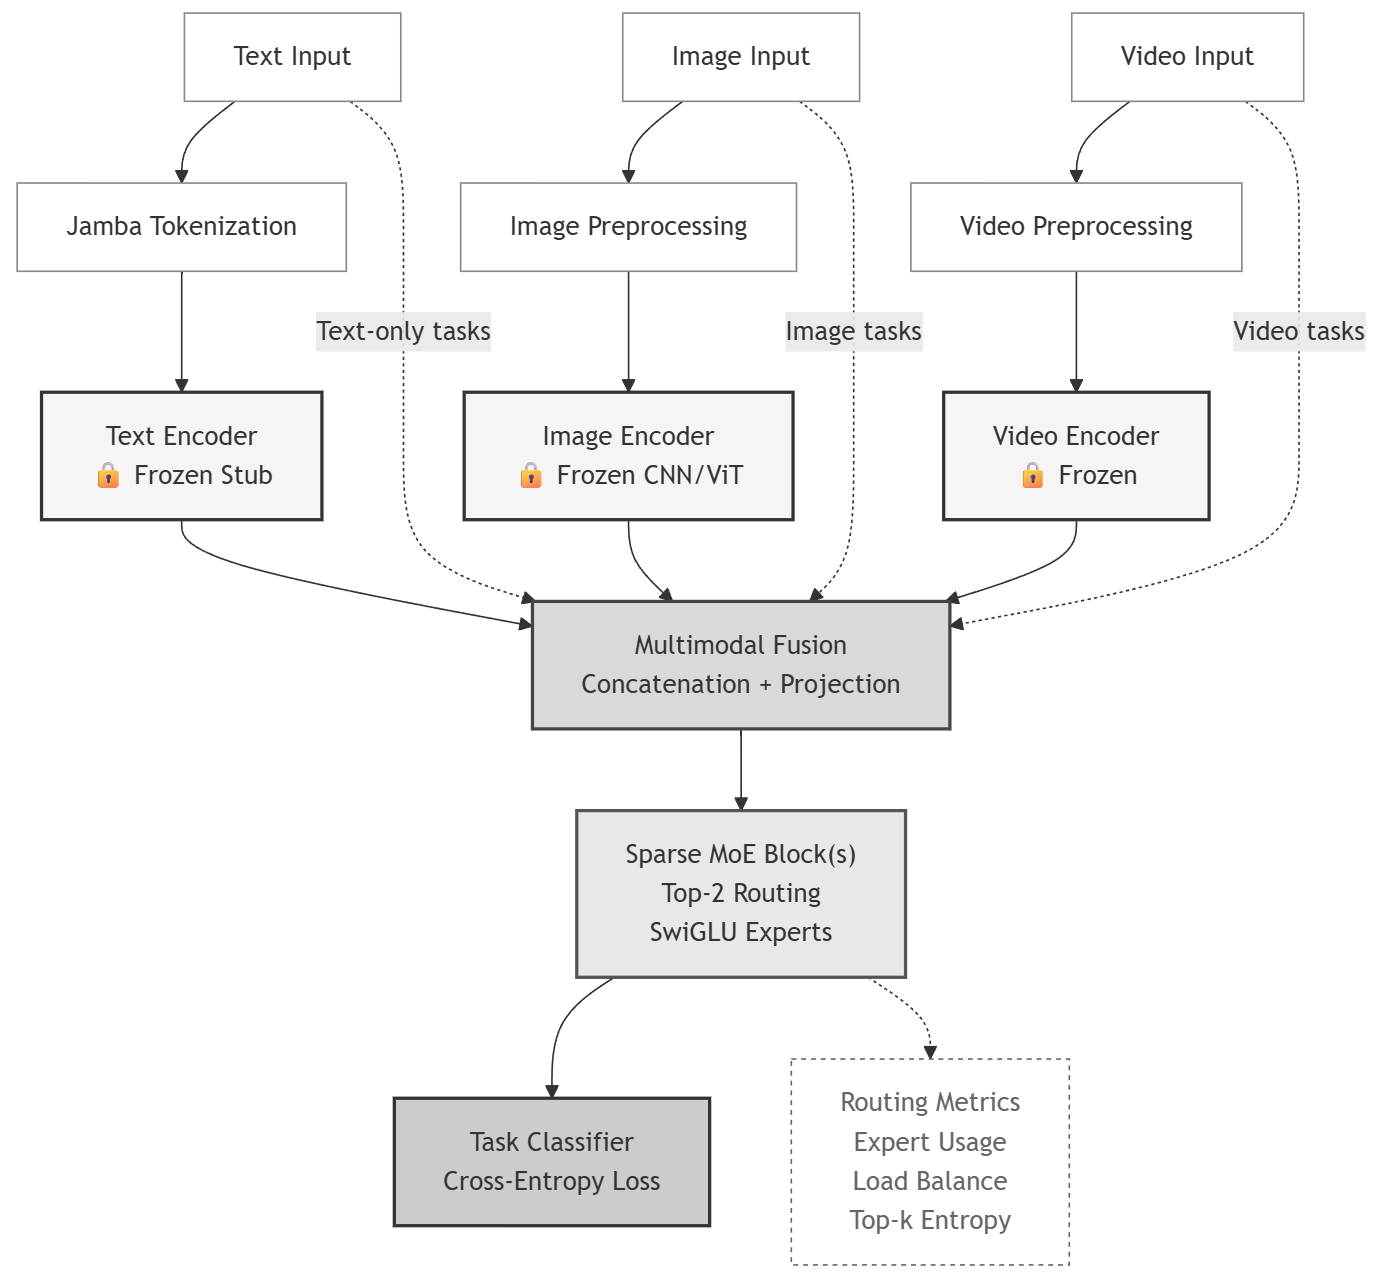
\includegraphics[width=\linewidth]{fig/poc_system_diagram.png}
  \caption{POC system diagram: inputs are tokenized/preprocessed and encoded by frozen modality encoders; embeddings are concatenated and projected; a Sparse MoE stack with top-2 routing (SwiGLU experts) processes the fused token; a classifier outputs task logits. Routing metrics (usage, load-balance, top-$k$ entropy) are recorded throughout training.}
  \label{fig:system-diagram}
\end{figure}

\subsection{Data Pipeline}
\begin{itemize}[leftmargin=*]
  \item Dataloaders for \CIFAR{}, \AGNEWS{}, and \MINIUCF{}.
  \item Per-batch logging of loss, expert counts, load-balance score, and top-$k$ entropy; per-run plots are generated by the evaluation utilities.
  \item Evaluation utilities generate: loss curves; balance/entropy trends per layer; expert usage bars and heatmaps.
\end{itemize}

\subsection{Fusion and MoE Details}
\textbf{Fusion.} Concatenate available modality embeddings (text/image/video) and project to a shared model dimension with layer normalization.

\textbf{Router.} A linear mapping produces expert logits; softmax yields mixture weights; top-2 experts are selected per sample with a capacity factor.

\textbf{Experts.} SwiGLU feed-forward modules. Layer normalization and residual connections wrap the MoE block.

\textbf{Metrics.}
\begin{itemize}[leftmargin=*]
\item Expert usage counts per batch and aggregated per epoch/phase.
\item Load-balance score across experts.
\item Top-$k$ entropy as a proxy for routing decisiveness.
\end{itemize}

\paragraph{Role of the Jamba tokenizer (ai21labs/Jamba-v0.1).}
Text is tokenized with the \href{https://huggingface.co/ai21labs/Jamba-v0.1}{ai21labs/Jamba-v0.1} tokenizer via \texttt{transformers} (\texttt{AutoTokenizer})\cite{jamba2024}. The POC does not load or fine-tune Jamba model weights: the text path is a frozen stub embedding that average-pools token embeddings under the attention mask. This preserves Jamba’s tokenization (vocabulary, special tokens, truncation/padding behavior) while avoiding LM compute, allowing us to isolate routing effects in the MoE. Consequently, tokenizer choice influences sequence lengths and token boundaries but does not confer pretrained language understanding; results should not be interpreted as Jamba model performance. See Appendix~C for the configuration fields \texttt{encoders.text.tokenizer\_name} and \texttt{encoders.text.stub=true}.

%==============================================================================
\section{Datasets}
\begin{table}[H]
\centering
\caption{POC datasets and usage. Replace placeholders with final counts after runs complete.}
\begin{tabularx}{\linewidth}{@{}l l c c c X@{}}
\toprule
Dataset & Modality & \#Classes & Train used & Val used \\
\midrule
\CIFAR{} & image + caption & 10 & 90\% of train & 10\% of train & Images resized to 224; captions derived from labels. \\
\AGNEWS{} & text & 4 & 2000 & 1000 & Max length 192; subset via HF splits. \\
\MINIUCF{} & video + caption & 2--4 & few/class & few/class & Frames 6--12; generated via \texttt{tools/make\_mini\_ucf.py}. \\
\bottomrule
\end{tabularx}
\end{table}

\paragraph{UCF101 to mini\_UCF preparation.}
The full UCF101 dataset is downloaded first. A partially downloaded subset is staged under \texttt{ucf101/} (classes/files available locally). The script \texttt{tools/make\_mini\_ucf.py} then constructs \texttt{data/mini\_ucf/\{train,val\}/\{Class\}/file.avi} by filtering UCF CSVs to present files, sampling a small number of clips per class, and linking/copying assets. The video loader reads uniformly sampled frames per clip, normalizes with ImageNet statistics, and pairs each clip with a lightweight caption template.

\paragraph{Exploratory analysis summaries.}
The following tables report class distributions observed in the exploratory notebook.

\begin{table}[H]
\centering
\caption{CIFAR-10 label distribution (train 90\%, val 10\%).}
\begin{tabular}{@{}r l r r r r@{}}
\toprule
Class & Name & Train Count & Val Count & Train \% & Val \% \\
\midrule
0 & airplane & 4500 & 500 & 10.0 & 10.0 \\
1 & automobile & 4486 & 514 & 10.0 & 10.3 \\
2 & bird & 4487 & 513 & 10.0 & 10.3 \\
3 & cat & 4470 & 530 & 9.9 & 10.6 \\
4 & deer & 4520 & 480 & 10.0 & 9.6 \\
5 & dog & 4551 & 449 & 10.1 & 9.0 \\
6 & frog & 4489 & 511 & 10.0 & 10.2 \\
7 & horse & 4485 & 515 & 10.0 & 10.3 \\
8 & ship & 4495 & 505 & 10.0 & 10.1 \\
9 & truck & 4517 & 483 & 10.0 & 9.7 \\
\midrule
\multicolumn{2}{r}{Total} & 45000 & 5000 & 100.0 & 100.0 \\
\bottomrule
\end{tabular}
\end{table}

\begin{table}[H]
\centering
\caption{AG News class distribution (train 2000, val 1000).}
\begin{tabular}{@{}r l r r r r@{}}
\toprule
Class & Name & Train Count & Val Count & Train \% & Val \% \\
\midrule
0 & World    & 477 & 268 & 23.8 & 26.8 \\
1 & Sports   & 338 & 274 & 16.9 & 27.4 \\
2 & Business & 408 & 205 & 20.4 & 20.5 \\
3 & Sci/Tech & 777 & 253 & 38.9 & 25.3 \\
\midrule
\multicolumn{2}{r}{Total} & 2000 & 1000 & 100.0 & 100.0 \\
\bottomrule
\end{tabular}
\end{table}

\begin{table}[H]
\centering
\caption{mini-UCF folder statistics (balanced 10 classes).}
\begin{tabular}{@{}r l r r r r@{}}
\toprule
Class & Name & Train Count & Val Count & Train \% & Val \% \\
\midrule
0 & Archery           & 8 & 4 & 10.0 & 10.0 \\
1 & Biking            & 8 & 4 & 10.0 & 10.0 \\
2 & CuttingInKitchen  & 8 & 4 & 10.0 & 10.0 \\
3 & GolfSwing         & 8 & 4 & 10.0 & 10.0 \\
4 & Knitting          & 8 & 4 & 10.0 & 10.0 \\
5 & PlayingGuitar     & 8 & 4 & 10.0 & 10.0 \\
6 & SkateBoarding     & 8 & 4 & 10.0 & 10.0 \\
7 & Surfing           & 8 & 4 & 10.0 & 10.0 \\
8 & TaiChi            & 8 & 4 & 10.0 & 10.0 \\
9 & YoYo              & 8 & 4 & 10.0 & 10.0 \\
\midrule
\multicolumn{2}{r}{Total} & 80 & 40 & 100.0 & 100.0 \\
\bottomrule
\end{tabular}
\end{table}

%==============================================================================
\section{Implementation}
\subsection{Libraries and Configuration}
PyTorch, torchvision, transformers, datasets, numpy, matplotlib; optional \texttt{av} for video decoding. Key knobs include epochs, batch sizes, learning rate, weight decay, shared hidden size, number of experts/layers, capacity factor, and frames per clip. Reproducibility uses fixed seeds; each run produces logs and plots and is listed in a global index with an accompanying summary CSV.
\textit{Text tokenization uses the fast} \texttt{ai21labs/Jamba-v0.1} \textit{tokenizer only (no LM weights are loaded); it is instantiated via} \texttt{AutoTokenizer.from\_pretrained} \textit{as specified in the config.}

\subsection{Training Strategy}
Encoders are frozen; optimization targets the fusion layer, MoE stack, and classifier head. AdamW is used with bfloat16 autocast when available (otherwise FP32). Gradient accumulation increases the effective batch. The loss is cross-entropy on task logits. The script \texttt{run\_different\_training\_scenarios.sh} orchestrates tasks and variants and invokes the evaluator to emit plots.

\subsection{Scenario sweep script}
The helper \texttt{run\_different\_training\_scenarios.sh} runs a matrix of tasks and ablations, producing per-run logs/plots and recording a global index and summary CSV:
\begin{itemize}[leftmargin=*]
  \item Tasks: \texttt{image\_text\_cifar10}, \texttt{text\_agnews}; \texttt{video\_folder} is added if the mini-UCF train/val folders are present.
  \item Scenarios (explicit overrides passed to the trainer):
  \begin{itemize}
    \item base: \#layers = 1, \#experts = 4, capacity = 1.25.
    \item ablation\_small: \#layers = 1, \#experts = 2, capacity = 1.25.
    \item ablation\_wide: \#layers = 2, \#experts = 8, capacity = 1.25.
    \item cap\_low: \#layers = 1, \#experts = 4, capacity = 1.00.
  \end{itemize}
  \item Intent only (POC constraints apply): base aims for a balanced reference; ablation\_small increases contention; ablation\_wide encourages specialization; cap\_low isolates capacity pressure.
\end{itemize}

\begin{table}[H]
\centering
\caption{Scenario hyperparameters. Unless noted, all other training settings follow the base configuration.}
\begin{tabular}{@{}l c c c c@{}}
\toprule
Hyperparameter & base & ablation\_small & ablation\_wide & cap\_low \\
\midrule
MoE layers (num\_layers)   & 1    & 1    & 2    & 1    \\
Experts (num\_experts)     & 4    & 2    & 8    & 4    \\
Capacity factor            & 1.25 & 1.25 & 1.25 & 1.00 \\
Top-$k$ (top\_k)           & 2    & 2    & 2    & 2    \\
Model dim (model\_dim)     & 1024 & 1024 & 1024 & 1024 \\
FFN dim (ffn\_dim)         & 4096 & 4096 & 4096 & 4096 \\
Router aux loss (weight)   & 0.03 & 0.03 & 0.03 & 0.03 \\
\bottomrule
\end{tabular}
\end{table}

%==============================================================================
\section{Evaluation}
\subsection{Metrics and Tables}
Primary metrics: train and validation loss per task and scenario. The experiment summary CSV (\texttt{checkpoints/summary\_runs.csv}) aggregates per-run last train/val losses and run descriptors. Accuracy is not computed in this sweep.

\begin{table}[H]
\centering
\caption{Summary of runs (last train/val loss).}
\begin{tabularx}{\linewidth}{@{}l l c c c c c X@{}}
\toprule
Task & Variant & Layers & Experts & Capacity & Last Train Loss & Val Loss \\
\midrule
\CIFAR{} & base & 1 & 4 & 1.25 & 4.1756e$-$07 & 2.0000e$-$06 & \\
\CIFAR{} & ablation\_small & 1 & 2 & 1.25 & 5.1527e$-$07 & 2.4311e$-$06 & \\
\CIFAR{} & ablation\_wide & 2 & 8 & 1.25 & 1.4634e$-$06 & 5.5999e$-$06 & \\
\CIFAR{} & cap\_low & 1 & 4 & 1 & 1.4722e$-$06 & 4.5667e$-$06 & \\
\AGNEWS{} & base & 1 & 4 & 1.25 & 0.0018 & 1.0748 & \\
\AGNEWS{} & ablation\_small & 1 & 2 & 1.25 & 0.0011 & 0.9736 & \\
\AGNEWS{} & ablation\_wide & 2 & 8 & 1.25 & 0.0038 & 1.4874 & \\
\AGNEWS{} & cap\_low & 1 & 4 & 1 & 0.0142 & 1.0862 & \\
\MINIUCF{} & base & 1 & 4 & 1.25 & 0.0003 & 0.0018 & \\
\MINIUCF{} & ablation\_small & 1 & 2 & 1.25 & 3.0110e$-$05 & 0.0002 & \\
\MINIUCF{} & ablation\_wide & 2 & 8 & 1.25 & 0.0001 & 0.0168 & \\
\MINIUCF{} & cap\_low & 1 & 4 & 1 & 0.0003 & 0.0018 & \\
\bottomrule
\end{tabularx}
\end{table}

\subsection{Plot roles}
\begin{itemize}[leftmargin=*]
  \item Loss curves: train averages vs. validation per-epoch loss; indicate optimization stability and under/overfitting gaps.
  \item Load-balance score: distributional evenness across experts; higher and steadier suggests healthier spread.
  \item Top-$k$ entropy: routing decisiveness among selected experts; lower indicates confident routing; spikes may reflect indecision or distribution shifts.
  \item Expert usage bars: per-epoch counts per expert; reveal monopolization vs. diversity.
  \item Expert usage heatmaps: batch-by-expert dynamics; expose mode collapse, rotation, or emerging specialization patterns.
\end{itemize}

\subsection{Ablation intents}
\begin{itemize}[leftmargin=*]
  \item base: balanced routing under moderate capacity; expect smooth losses and healthy balance.
  \item ablation\_small: minimal MoE capacity to test contention; expect skewed counts and lower balance.
  \item ablation\_wide: larger expert pool and deeper MoE; expect more diverse usage and potentially lower entropy.
  \item cap\_low: capacity stress without changing topology; expect capped per-batch counts and more overflow pressure.
\end{itemize}

%==============================================================================
\section{Results}
We report loss trajectories and routing instrumentation per task and scenario. For each scenario: loss curves are shown separately; expert heatmaps are visualized as grids of single-epoch images per split (train/val); expert usage remains stacked (train top, val bottom).

\subsection{CIFAR-10 (image+text)}
\subsubsection*{base (1 layer, 4 experts, cap 1.25)}
\begin{figure}[H]
  \centering
  \includegraphics[width=\LossCurvesScale\linewidth]{fig/cifar10/base/loss_curves.png}
  \caption{CIFAR-10 base: loss curves (train average and validation per epoch).}
\end{figure}
% single-image grids
\HeatmapGridOneLayer{fig/cifar10/base}{train}{0}{CIFAR-10 base: expert heatmaps (train, epochs 1–10, layer 0).}
\HeatmapGridOneLayer{fig/cifar10/base}{val}{0}{CIFAR-10 base: expert heatmaps (val, epochs 1–10, layer 0).}
% expert usage stacked
\begin{figure}[H]
  \centering
  \includegraphics[width=\linewidth]{fig/cifar10/base/expert_usage_epochs_overview_train.png}\\[0.5em]
  \includegraphics[width=\linewidth]{fig/cifar10/base/expert_usage_epochs_overview_val.png}
  \caption{CIFAR-10 base: expert usage across epochs (train top, val bottom).}
\end{figure}

\subsubsection*{ablation\_small (1 layer, 2 experts, cap 1.25)}
\begin{figure}[H]
  \centering
  \includegraphics[width=\LossCurvesScale\linewidth]{fig/cifar10/ablation_small/loss_curves.png}
  \caption{CIFAR-10 ablation\_small: loss curves.}
\end{figure}
\HeatmapGridOneLayer{fig/cifar10/ablation_small}{train}{0}{CIFAR-10 ablation\_small: expert heatmaps (train, layer 0).}
\HeatmapGridOneLayer{fig/cifar10/ablation_small}{val}{0}{CIFAR-10 ablation\_small: expert heatmaps (val, layer 0).}
\begin{figure}[H]
  \centering
  \includegraphics[width=\linewidth]{fig/cifar10/ablation_small/expert_usage_epochs_overview_train.png}\\[0.5em]
  \includegraphics[width=\linewidth]{fig/cifar10/ablation_small/expert_usage_epochs_overview_val.png}
  \caption{CIFAR-10 ablation\_small: expert usage (train top, val bottom).}
\end{figure}

\subsubsection*{ablation\_wide (2 layers, 8 experts, cap 1.25)}
\begin{figure}[H]
  \centering
  \includegraphics[width=\LossCurvesScale\linewidth]{fig/cifar10/ablation_wide/loss_curves.png}
  \caption{CIFAR-10 ablation\_wide: loss curves.}
\end{figure}
\HeatmapGridTwoLayers{fig/cifar10/ablation_wide}{train}{CIFAR-10 ablation\_wide: expert heatmaps (train, layers 0–1).}
\HeatmapGridTwoLayers{fig/cifar10/ablation_wide}{val}{CIFAR-10 ablation\_wide: expert heatmaps (val, layers 0–1).}
\begin{figure}[H]
  \centering
  \includegraphics[width=\linewidth]{fig/cifar10/ablation_wide/expert_usage_epochs_overview_train.png}\\[0.5em]
  \includegraphics[width=\linewidth]{fig/cifar10/ablation_wide/expert_usage_epochs_overview_val.png}
  \caption{CIFAR-10 ablation\_wide: expert usage (train top, val bottom).}
\end{figure}

\subsubsection*{cap\_low (1 layer, 4 experts, cap 1.00)}
\begin{figure}[H]
  \centering
  \includegraphics[width=\LossCurvesScale\linewidth]{fig/cifar10/cap_low/loss_curves.png}
  \caption{CIFAR-10 cap\_low: loss curves.}
\end{figure}
\HeatmapGridOneLayer{fig/cifar10/cap_low}{train}{0}{CIFAR-10 cap\_low: expert heatmaps (train, layer 0).}
\HeatmapGridOneLayer{fig/cifar10/cap_low}{val}{0}{CIFAR-10 cap\_low: expert heatmaps (val, layer 0).}
\begin{figure}[H]
  \centering
  \includegraphics[width=\linewidth]{fig/cifar10/cap_low/expert_usage_epochs_overview_train.png}\\[0.5em]
  \includegraphics[width=\linewidth]{fig/cifar10/cap_low/expert_usage_epochs_overview_val.png}
  \caption{CIFAR-10 cap\_low: expert usage (train top, val bottom).}
\end{figure}

% AG News
\subsection{AG News (text)}
\subsubsection*{base (1 layer, 4 experts, cap 1.25)}
\begin{figure}[H]
  \centering
  \includegraphics[width=\LossCurvesScale\linewidth]{fig/agnews/base/loss_curves.png}
  \caption{AG News base: loss curves.}
\end{figure}
\HeatmapGridOneLayer{fig/agnews/base}{train}{0}{AG News base: expert heatmaps (train, layer 0).}
\HeatmapGridOneLayer{fig/agnews/base}{val}{0}{AG News base: expert heatmaps (val, layer 0).}
\begin{figure}[H]
  \centering
  \includegraphics[width=\linewidth]{fig/agnews/base/expert_usage_epochs_overview_train.png}\\[0.5em]
  \includegraphics[width=\linewidth]{fig/agnews/base/expert_usage_epochs_overview_val.png}
  \caption{AG News base: expert usage (train top, val bottom).}
\end{figure}

\subsubsection*{ablation\_small (1 layer, 2 experts, cap 1.25)}
\begin{figure}[H]
  \centering
  \includegraphics[width=\LossCurvesScale\linewidth]{fig/agnews/ablation_small/loss_curves.png}
  \caption{AG News ablation\_small: loss curves.}
\end{figure}
\HeatmapGridOneLayer{fig/agnews/ablation_small}{train}{0}{AG News ablation\_small: expert heatmaps (train, layer 0).}
\HeatmapGridOneLayer{fig/agnews/ablation_small}{val}{0}{AG News ablation\_small: expert heatmaps (val, layer 0).}
\begin{figure}[H]
  \centering
  \includegraphics[width=\linewidth]{fig/agnews/ablation_small/expert_usage_epochs_overview_train.png}\\[0.5em]
  \includegraphics[width=\linewidth]{fig/agnews/ablation_small/expert_usage_epochs_overview_val.png}
  \caption{AG News ablation\_small: expert usage (train top, val bottom).}
\end{figure}

\subsubsection*{ablation\_wide (2 layers, 8 experts, cap 1.25)}
\begin{figure}[H]
  \centering
  \includegraphics[width=\LossCurvesScale\linewidth]{fig/agnews/ablation_wide/loss_curves.png}
  \caption{AG News ablation\_wide: loss curves.}
\end{figure}
\HeatmapGridTwoLayers{fig/agnews/ablation_wide}{train}{AG News ablation\_wide: expert heatmaps (train, layers 0–1).}
\HeatmapGridTwoLayers{fig/agnews/ablation_wide}{val}{AG News ablation\_wide: expert heatmaps (val, layers 0–1).}
\begin{figure}[H]
  \centering
  \includegraphics[width=\linewidth]{fig/agnews/ablation_wide/expert_usage_epochs_overview_train.png}\\[0.5em]
  \includegraphics[width=\linewidth]{fig/agnews/ablation_wide/expert_usage_epochs_overview_val.png}
  \caption{AG News ablation\_wide: expert usage (train top, val bottom).}
\end{figure}

\subsubsection*{cap\_low (1 layer, 4 experts, cap 1.00)}
\begin{figure}[H]
  \centering
  \includegraphics[width=\LossCurvesScale\linewidth]{fig/agnews/cap_low/loss_curves.png}
  \caption{AG News cap\_low: loss curves.}
\end{figure}
\HeatmapGridOneLayer{fig/agnews/cap_low}{train}{0}{AG News cap\_low: expert heatmaps (train, layer 0).}
\HeatmapGridOneLayer{fig/agnews/cap_low}{val}{0}{AG News cap\_low: expert heatmaps (val, layer 0).}
\begin{figure}[H]
  \centering
  \includegraphics[width=\linewidth]{fig/agnews/cap_low/expert_usage_epochs_overview_train.png}\\[0.5em]
  \includegraphics[width=\linewidth]{fig/agnews/cap_low/expert_usage_epochs_overview_val.png}
  \caption{AG News cap\_low: expert usage (train top, val bottom).}
\end{figure}

% mini-UCF
\subsection{mini-UCF (video+text)}
\subsubsection*{base (1 layer, 4 experts, cap 1.25)}
\begin{figure}[H]
  \centering
  \includegraphics[width=\LossCurvesScale\linewidth]{fig/mini_ucf/base/loss_curves.png}
  \caption{mini-UCF base: loss curves.}
\end{figure}
\HeatmapGridOneLayer{fig/mini_ucf/base}{train}{0}{mini-UCF base: expert heatmaps (train, layer 0).}
\HeatmapGridOneLayer{fig/mini_ucf/base}{val}{0}{mini-UCF base: expert heatmaps (val, layer 0).}
\begin{figure}[H]
  \centering
  \includegraphics[width=\linewidth]{fig/mini_ucf/base/expert_usage_epochs_overview_train.png}\\[0.5em]
  \includegraphics[width=\linewidth]{fig/mini_ucf/base/expert_usage_epochs_overview_val.png}
  \caption{mini-UCF base: expert usage (train top, val bottom).}
\end{figure}

\subsubsection*{ablation\_small (1 layer, 2 experts, cap 1.25)}
\begin{figure}[H]
  \centering
  \includegraphics[width=\LossCurvesScale\linewidth]{fig/mini_ucf/ablation_small/loss_curves.png}
  \caption{mini-UCF ablation\_small: loss curves.}
\end{figure}
\HeatmapGridOneLayer{fig/mini_ucf/ablation_small}{train}{0}{mini-UCF ablation\_small: expert heatmaps (train, layer 0).}
\HeatmapGridOneLayer{fig/mini_ucf/ablation_small}{val}{0}{mini-UCF ablation\_small: expert heatmaps (val, layer 0).}
\begin{figure}[H]
  \centering
  \includegraphics[width=\linewidth]{fig/mini_ucf/ablation_small/expert_usage_epochs_overview_train.png}\\[0.5em]
  \includegraphics[width=\linewidth]{fig/mini_ucf/ablation_small/expert_usage_epochs_overview_val.png}
  \caption{mini-UCF ablation\_small: expert usage (train top, val bottom).}
\end{figure}

\subsubsection*{ablation\_wide (2 layers, 8 experts, cap 1.25)}
\begin{figure}[H]
  \centering
  \includegraphics[width=\LossCurvesScale\linewidth]{fig/mini_ucf/ablation_wide/loss_curves.png}
  \caption{mini-UCF ablation\_wide: loss curves.}
\end{figure}
\HeatmapGridTwoLayers{fig/mini_ucf/ablation_wide}{train}{mini-UCF ablation\_wide: expert heatmaps (train, layers 0–1).}
\HeatmapGridTwoLayers{fig/mini_ucf/ablation_wide}{val}{mini-UCF ablation\_wide: expert heatmaps (val, layers 0–1).}
\begin{figure}[H]
  \centering
  \includegraphics[width=\linewidth]{fig/mini_ucf/ablation_wide/expert_usage_epochs_overview_train.png}\\[0.5em]
  \includegraphics[width=\linewidth]{fig/mini_ucf/ablation_wide/expert_usage_epochs_overview_val.png}
  \caption{mini-UCF ablation\_wide: expert usage (train top, val bottom).}
\end{figure}

\subsubsection*{cap\_low (1 layer, 4 experts, cap 1.00)}
\begin{figure}[H]
  \centering
  \includegraphics[width=\LossCurvesScale\linewidth]{fig/mini_ucf/cap_low/loss_curves.png}
  \caption{mini-UCF cap\_low: loss curves.}
\end{figure}
\HeatmapGridOneLayer{fig/mini_ucf/cap_low}{train}{0}{mini-UCF cap\_low: expert heatmaps (train, layer 0).}
\HeatmapGridOneLayer{fig/mini_ucf/cap_low}{val}{0}{mini-UCF cap\_low: expert heatmaps (val, layer 0).}
\begin{figure}[H]
  \centering
  \includegraphics[width=\linewidth]{fig/mini_ucf/cap_low/expert_usage_epochs_overview_train.png}\\[0.5em]
  \includegraphics[width=\linewidth]{fig/mini_ucf/cap_low/expert_usage_epochs_overview_val.png}
  \caption{mini-UCF cap\_low: expert usage (train top, val bottom).}
\end{figure}
%==============================================================================
\section{Discussion}
\textbf{Challenges.} Frozen encoders cap accuracy; video IO constrains batch sizes; capacity tuning trades off throughput and balance.

\textbf{Insights.} Load-balance stability tends to correlate with lower validation loss across scenarios; entropy spikes often accompany heterogeneous batches; expert preferences per class can emerge in longer runs.

\textbf{Ablation takeaways.} More experts/layers spread routing and can reduce loss; reduced capacity stresses routing and may harm validation loss. These are intents in a POC setting; observed magnitudes depend on runtime limits.

\subsection*{Cross-scenario considerations (executive summary)}
\begin{itemize}[leftmargin=*]
  \item Frozen encoders with sparse MoE learn useful decision boundaries rapidly; the ceiling is set by representation quality and routing design. Validation improvements typically plateau once the fused-token representation is exhausted.
  \item MoE size is not a free win under short budgets and a single routed token. Smaller or moderate MoE often generalizes better than very wide MoE in this regime.
  \item Capacity matters primarily when it binds. With small effective batches and one fused token, lowering capacity has limited effect; higher capacity helps mainly when expert slots saturate.
\end{itemize}

\subsection*{Task-level conclusions (intent-focused)}
\textbf{AG News (text-only).}
\begin{itemize}[leftmargin=*]
  \item Best validation typically occurs early; continued training trends toward overfitting due to the frozen stub text pathway.
  \item MoE variations shift when the plateau arrives rather than preventing overfit. Early stopping is recommended; width and capacity adjustments do not substitute for a stronger text encoder.
\end{itemize}

\textbf{CIFAR-10 (image + label-derived captions).}
\begin{itemize}[leftmargin=*]
  \item All scenarios converge trivially because captions encode the class name, collapsing task difficulty.
  \item Use CIFAR-10 primarily to validate routing instrumentation. For meaningful comparisons, evaluate with neutral captions (e.g., “a photo”) or image-only to remove leakage.
\end{itemize}

\textbf{mini-UCF (video + simple text).}
\begin{itemize}[leftmargin=*]
  \item Moderate or small MoE configurations provide stable specialization and strong late-phase improvements under the current budget and frozen encoders.
  \item Very wide MoE increases competition and assignment churn; benefits may diminish without more tokens, batches, or training time. Capacity reductions had little impact because slots were not saturated.
\end{itemize}

\subsection*{Practical guidance for this POC}
\begin{itemize}[leftmargin=*]
  \item Prefer moderate MoE (layers/experts) for fused-token routing with frozen encoders; add width only if expert slots are demonstrably saturated.
  \item Tune capacity upward only when counts indicate binding; otherwise expect minimal change. To surface capacity effects, increase batch or routed tokens.
  \item Select checkpoints by validation loss with early stopping on text-only; for CIFAR-10 and video, final-epoch checkpoints are acceptable when validation continues to improve.
\end{itemize}

%==============================================================================
\section{Disclaimer}
Consistent with the project guidelines, generative AI assistance was employed for code scaffolding, report drafting, and documentation generation. All produced code and scripts have been reviewed, executed, and verified for correctness within the project environment. Experimental results, figures, and configurations were validated against the logged runs and summary artifacts.

%==============================================================================
\section{Conclusion and Future Work}
This POC achieves a minimal multimodal Sparse MoE with interpretable routing and reproducible, scripted ablations across three modalities. Future work includes replacing the text stub with a real encoder, using CLIP/ViT and a lightweight video backbone, partial unfreezing, explicit router regularization, temporal experts, and longer training on larger datasets.

%==============================================================================
\section*{Appendices}
\subsection*{A. Reproducibility}
Hardware, CUDA/PyTorch versions, seeds. A run index and a summary CSV are produced during sweeps. Per-run resolved configs are stored alongside the run outputs. The notebooks visualize results and export figures for insertion.

\subsection*{B. Commands}
\begin{verbatim}
# runs automated training experiments across the different scenarios
./run_different_training_scenarios.sh

# evaluate specific run
python -m src.evaluation.eval_poc --run_dir <RUN_DIR>
\end{verbatim}

\subsection*{C. Full training configuration (config.yaml)}
\begin{verbatim}
base: &base
  seed: 42
  task: "image_text_cifar10" # options: image_text_cifar10, text_agnews, video_folder
  output_dir: "checkpoints/poc"
  num_epochs: 10
  per_device_train_batch_size: 64
  per_device_eval_batch_size: 64
  learning_rate: 1e-4
  weight_decay: 0.01
  bf16: true
  log_every: 25
  grad_accum_steps: 4
  save_checkpoints: false  # by default, don't save .pt files to save storage

data:
  image:
    image_size: 224
    train_split: "train[:90%]"
    val_split:   "train[90%:]"
  text:
    dataset_name: "ag_news" # small, quick
    train_split: "train[:2000]"
    val_split:   "test[:1000]"
    max_length: 192
  video:
    root: "data/mini_ucf" # path to folder with video files
    image_size: 224
    num_frames: 12
    max_text_len: 16
    batch_size_train: 2
    batch_size_eval: 4

encoders:
  text:
    tokenizer_name: "ai21labs/Jamba-v0.1"
    hidden_size: 1536
    frozen: true
    stub: true
  image:
    proj_out: 1536
    frozen: true
  video:
    proj_out: 1536 
    frozen: true

fusion:
  hidden_size: 1536

moe:
  num_layers: 2
  model_dim: 1024
  ffn_dim: 4096
  activation: "swiglu"
  num_experts: 4
  top_k: 2
  capacity_factor: 2.0
  router_aux_loss_weight: 0.03

# tiny ablations
ablation_small:
  <<: *base
  output_dir: "checkpoints/ablation_small"
  moe:
    num_layers: 1
    num_experts: 2

ablation_wide:
  <<: *base
  output_dir: "checkpoints/ablation_wide"
  moe:
    num_layers: 2
    num_experts: 8
\end{verbatim}

%==============================================================================
% References 
% \bibliographystyle{unsrt}
% \bibliography{references}
\printbibliography

\end{document}